\documentclass[12pt,a4paper]{report}

%packages
\usepackage{eso-pic}
\usepackage{xcolor}
\usepackage[textwidth=17cm,textheight=24cm, bindingoffset=1.2cm]{geometry}
\usepackage{amsmath}
\usepackage{amsfonts}
\usepackage{amssymb}
\usepackage{amsrefs}
\usepackage{graphicx}
\usepackage{fancyhdr}
\usepackage[Glenn]{fncychap}
\usepackage{amsthm}
\usepackage{fourier}
\usepackage[colorlinks=true]{hyperref}
\usepackage[utf8]{inputenc}

%mathdef
\theoremstyle{plain}
\newtheorem{Conj}{Conjecture}
\newtheorem{Def}{Definition}[chapter]
\newtheorem{Ex}{Example}[chapter]
\newtheorem{Theo}{Theorem}[chapter]
\newtheorem{Pro}{Proposition}[chapter]
\newtheorem{Coro}{Corollary}[chapter]
\newtheorem{Lem}{Lemma}[chapter]
\newtheorem{Rem}{Remark}[chapter]

%newcommand
\newcommand{\al}{\alpha}
\newcommand{\te}{\theta}
\newcommand{\sq}{\sqrt}
\newcommand{\N}{\mathbb{N}}
\newcommand{\Z}{\mathbb{Z}}
\newcommand{\Q}{\mathbb{Q}}
\newcommand{\R}{\mathbb{R}}
\newcommand{\C}{\mathbb{C}}
\newcommand\BackgroundPic{\put(0,0){\parbox[b][\paperheight]{\paperwidth}{ 
\vfill
\centering
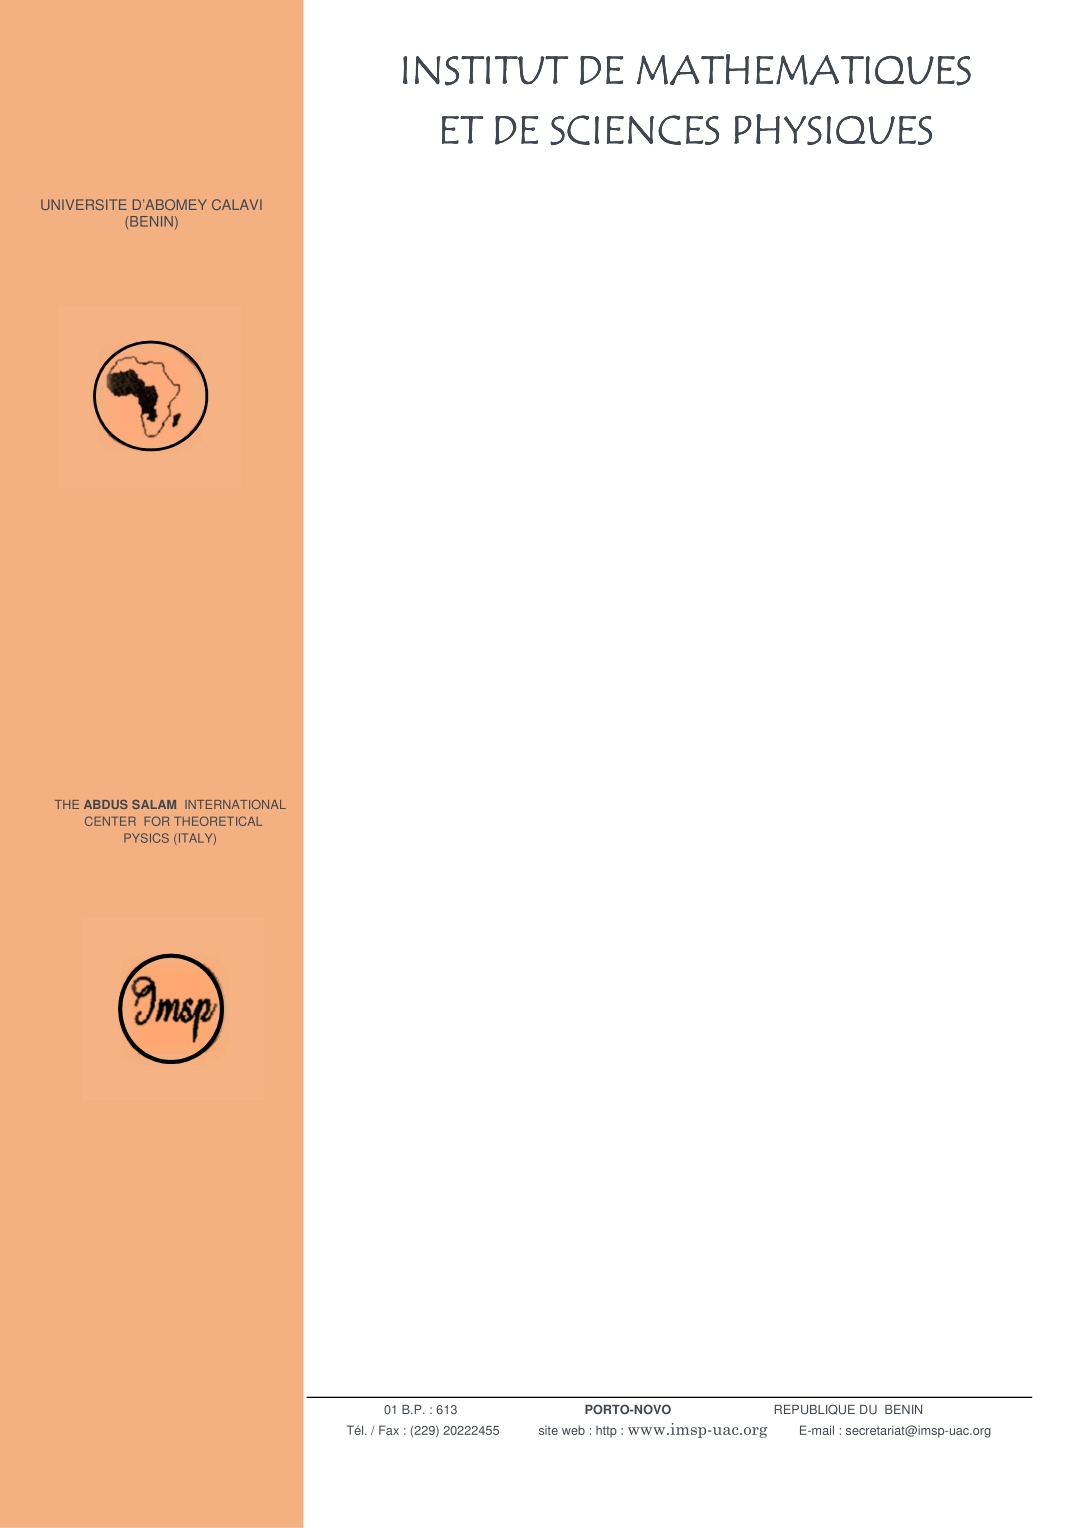
\includegraphics[width=\paperwidth,height=\paperheight]{Image1.jpeg}
\vfill}}}

%mise en page
\fancypagestyle{plain}{%
  \fancyhf{} %
  \fancyfoot[L]{\textbf{\small Schémas monotones discrets pour l'équation de Schrödinger}} %
  \fancyfoot[C]{} %
  \fancyfoot[R]{\thepage}%
  \renewcommand{\headrulewidth}{0pt}
  \renewcommand{\footrulewidth}{1pt}}
\pagestyle{fancy}
\fancyhead[L]{\leftmark}
\fancyhead[R]{\thepage}
\fancyfoot[L]{\nouppercase{\bfseries{\rightmark}}}
\fancyfoot[C]{}
\fancyfoot[R]{\textbf{\small Schémas monotones discrets pour l'équation de Schrödinger}}
\renewcommand{\headrulewidth}{0.7pt}
\renewcommand{\footrulewidth}{0.7pt}
\pagenumbering{roman}


\begin{document}
	
	%$$$$$$$$$$$$$$$$$$$$$$$$$$$$$$$$$$
	%Premiere page du documet
	%$$$$$$$$$$$$$$$$$$$$$$$$$$$$$$$$$$
	
	%mise en place du fond de page d l'imsp 
	\AddToShipoutPictureBG*{\BackgroundPic}
	
	%mise en place le page de garde
	\newgeometry{top=3.75cm,bottom=2cm,left=6.8cm,right=1cm}
	\thispagestyle{empty}
	\rule{12.3cm}{0.1cm}
	\vspace{1cm}
	\begin{center}
		{\bfseries {\Large M}\'EMOIRE DE {\Large M}ASTER}\\
		Math\'ematiques Fondamentales et Applications\\
	\end{center}
	%\begin{center}
		%{\Large S}P\'ECIALIT\'E\\
		%Recherche Opérationnelle
	%\end{center}
	\vspace{2.5cm}
	\begin{center}\setlength{\unitlength}{1cm}
	\begin{picture}(0,0)		\linethickness{1pt}
	\put(-0.98,0.68){\fontsize{15.3}{15.3}\selectfont \bfseries TH\`EME}
	\put(-6.5,-0.68){\fontsize{14.5}{18.5}\selectfont \bfseries Schémas monotones discrets pour l'équation de Schrödinger}
	\end{picture}
	\end{center}
	\vspace{2.5cm}
	\begin{flushright}
	\large Superviseur:\\
	{\color{orange}{Prof. Julien SALOMON}}\\
	Sorbonne Université, UPMC Univ Paris 06,\\
	UMR 7598, Laboratoire Jacques-Louis Lions,\\
	Paris, France
 	\end{flushright}
	\vspace{2.5cm}
	\begin{center}
		{\bfseries Rédigé  par:}\\
		{\color{orange}{\large Kenneth 0. ASSOGBA\\ }}\
		kennethassogba@gmail.com \\
		
	\end{center}
	\vspace{2.5cm}
	\begin{center}
		Ann\'ee Acad\'emique: 2018-2019
	\end{center}
	\restoregeometry

\end{document}

